\chapter{State of the Art}\label{chapter:c2}
\markboth{Chapter~\ref{chapter:c2}. State of the Art}{}
In this chapter, it will be introduced the state-of-the-art 
related to the specification, formalization and verfication
of stateful web services and their composition as well as the use of formal methods in this topic. The aim of this chapter is to provide the reader
with the basic notions about formal methods and stateful web service compositions in order to help he/she in the understanding
of the Thesis. To begin with, a brief introduction of formal methods 
and why they are needed is presented. Second, a survey about the diffent technologies used to model web services
and the different approaches to compose them are introduced and,
next, the different mechanisms available to improve
these web services with distributed resources. 
Finally, the different formal models used here are defined. 
On the other hand, we introduce workflow nets
and why they are useful to model business processess. 
Some informal definition about the properties can be studied with this formal model is also provided. 

\section{Motivation}

Throughout the history of computing , engineers and researchers have used different formal methods to improve the quality of hardware and software. These systems with continuous technological progress in integration techniques and programming methodologies inevitably grow in scale and complexity. Because of this complexity, the probability of error is higher and, in addition, some of these errors can cause incalculable economic losses, time or even the loss of human lives. Therefore, the main aim of designers should be to provide developers with the required tools to build systems with a negligible error rate and with the lowest cost. However, this task is far from trivial since one needs to ensure the correctness of the specifications and needs to provide techniques that ease error detection and the verification of the developed models without consuming so much time of the development process. One of the ways that engineers have been used to achieve this goal is the use of formal techniques to ensure the correctness of the development process as well as the product under construction. These formal methods can be defined as the set of procedures and tools based on mathematical languages that virtually ensure the correctness of a system \cite{Clarke96} since they increase the level of knowledge that the participants have about the system, revealing inconsistencies and ambiguities that could not be detected using other techniques, i.e., the use of formal methods provides a greater degree of refinement of the model than other methods.


\begin{figure}
\begin{center}
  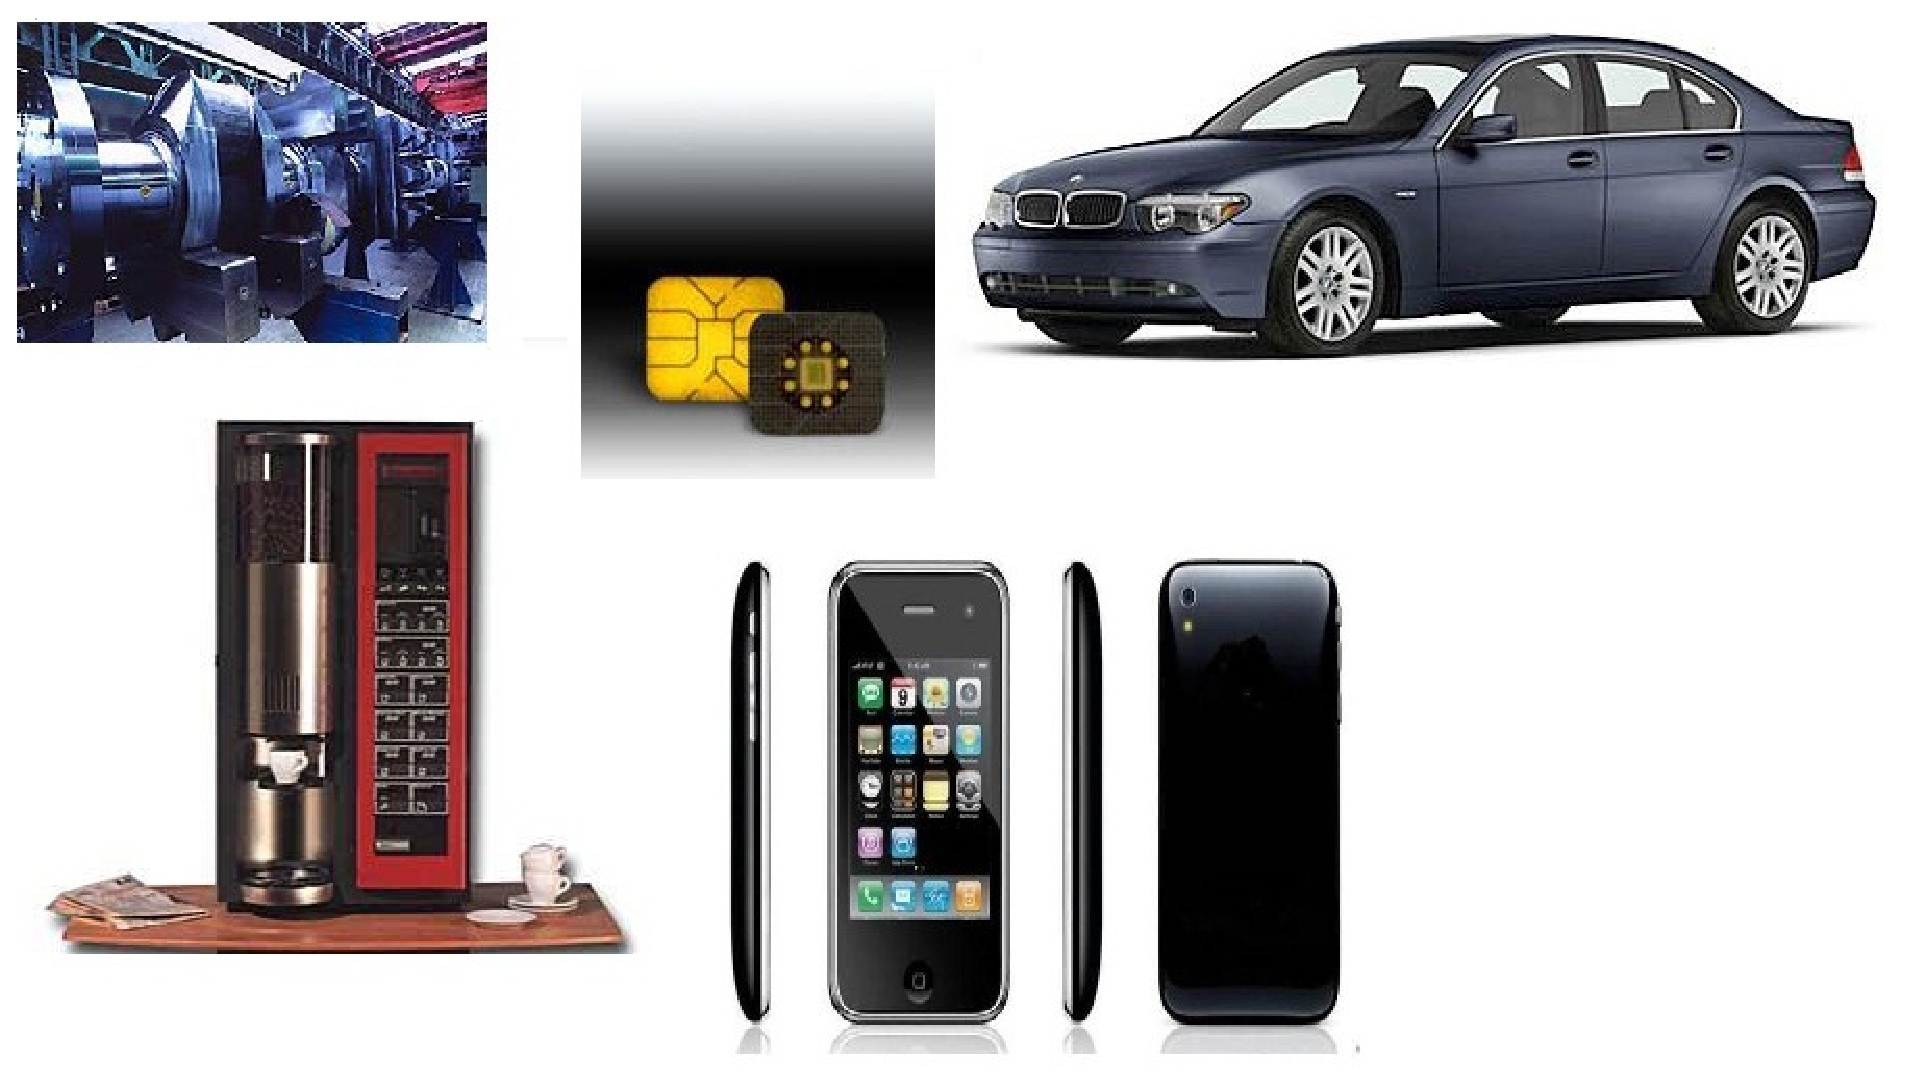
\includegraphics[scale=0.5, width =\columnwidth]{Figures/usos}
\end{center}
  \caption{Example of systems where formal methods are (can be) used .}
  \label{fig:uso}
\end{figure}

In the past, the use of formal techniques in practice seemed to be utopian and unrealizable. 
Among other causes, the notations used to require a high mathematical background in
mathematics and, therefore, they were too complicated for the uninitiated in the topic. 
The techniques did not allow the system to be scalable and the existing tools were
too difficult to use or understand or even there were no tools for a particular 
technique or formalism. In addition, case studies were not convincing enough and, 
therefore, developers could not appreciate the usefulness of formalization. 
However, in the early 90s, it started to glimpse a new way in this area. 
For the specification of software, the industry began to use the language Z \cite{Abrial80} 
in order to obtain rigorous specifications. For hardware verification, major 
companies such as Intel and AMD started to use formal techniques such as \emph{model checking} 
or \emph{theorem proving} to supplement tests on simulators. This led to the description of larger case studies,
which was benefitial for the advance of this area since other developers started to consider the possibility of 
introducing the use of formal techniques into their development processes.
In Figure \ref{fig:uso}, one can observe different systems in which these techniques are currently
used to ensure proper operation. For instance, big companies (e.g Boeing and Airbus)
use formal languages to specify the requirements of the equipment as well as they use 
formal methods to verify the most critical systems in the aircrafts. Moreover, automotive
companies verify the most critical systems ( e.g. brake or airbag systems) using \emph{model checking}. 

The main advantages of using formal methods are:

\begin{itemize}
\item The use of mathematics as a base gives this approach a certain rigour.
\item Identify ambiguity and inconsistencies.
\item Facilitates the construction of consistent and \emph{deadlock-free} systems.
\item Provides customer confidence in the system.
\item There are many tools that support the existing techniques.
\item Find bugs early should save money.
\end{itemize} 

The main disadvantages (or beliefs) that slow the progress of this area are:

\begin{itemize}
\item It is believed that the use of formal methods slows the development process.
\item Many developers think it is difficult to work with formal specifications.
\item It does not guarantee the correctness of the implemented code (only the model
it is based).
\item Increasing system complexity causes an exponential increase
the complexity of the verification.
\end{itemize}

As commented previously, companies can use formal methods along the entire
development lifecycle of a system, both hardware and software. 
Here, we will focus on software since this Thesis studies different standards for building software components. 
Next, we describe the different phases in which designers can apply any formal technique. 

One of the most important part in the development of a system is the requirements specification. 
A specification can be seen as a technical document where the features and services needed 
to build a product are stated. Nevertheless, it can also include information on 
subsequent steps such as verification, validation, testing, etc. Therefore, 
this should be the first part in which the participants should apply formal methods, taking the 
required time to correctly specify the system since a neat and correct specification will influence the 
rest of the proccess.
Anyway, make a proper specification does not guarantee the absence of errors because the 
presence of faults is an intrinsic characteristic of the systems. In this sense, 
the simple act of writing the document helps engineers to find errors in the early stages 
of the development process, helping the company to save  money and time. 
In Figure \ref{fig:coste}, one can observe what is the effect (in money) of finding a bug
in the different phases. As can be observed, the cost of fixing a bug increases as 
we advance in the lifecycle and, therefore, it is recommended to find these bugs as soon as possible. 
In this Thesis, we propose a formal language and its visual model to specify web service compositions 
with distributed resources, but this will be presented in Chapter \ref{chapter:c3}.

\begin{figure}
\begin{center}
  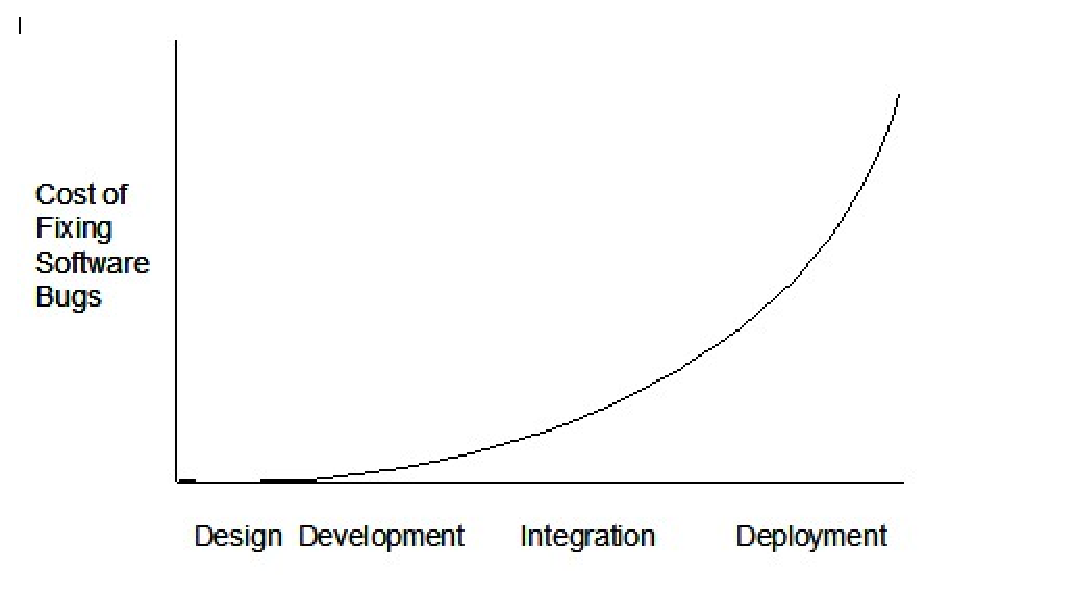
\includegraphics[scale=0.5, width =\columnwidth]{Figures/coste}
\end{center}
  \caption{Cost evolution of fixing a bug.}
  \label{fig:coste}
\end{figure}

In the classic life cycle, the verification and validation phases are performed after the implementation phase, 
but as we have seen in Figure \ref{fig:coste}, it is advisable to detect these errors as soon as possible. 
As expected, it is practically impossible to verify completely all the behaviour of a complex 
system so that the goal of researchers in this area is to check whether certain properties hold in the model. 
The properties of interest will be related to the classical problems of concurrency (\emph{deadlock, mutual exclusion,\ldots}) 
and some aspects directly related to the system itself such as check 
the adherence of it to certain time constraints. For example, in a banking system, 
it is mandatory to ensure that transactions meet the stipulated time for completion 
because if you exceed these restrictions some security issues could come out.

In this sense, one can follow two different ways to perform 
the verification of a system: \emph{Human-directed proof or Automated proof}.
The first one is used when you want to strengthen the knowledge of the system 
rather than completely ensure the correctness of it, and, therefore, it is a person who check the properties manually. 
This variant improves the knowledge of the system, but it is time-consuming and 
error-prone due to the entire process is conducted for a human being. 
In the second approach (\emph{automated proof}) there are also two variants: \emph{automated theorem proving and model checking}. 
The \emph{automated theorem proving } is conducted by a program that tries 
to produce a formal proof of a system from scratch, giving a description of it, 
a set of logical axioms and a set of inference rules. On the other hand, model checking \cite{Clarke99} 
is a technique for verifying finite state concurrent systems. It has a number of advantages 
over traditional approaches that are based on simulation, testing, and deductive reasoning. 
In particular, model checking is normally automatic and usually quite fast. Also, if the design contains an error, 
model checking will produce a counterexample that can be used to pinpoint the source of the error. 
Here, the specification can be expressed in propositional temporal logic propositional 
normally LTL \cite{Pnueli77} or CTL \cite{Henzinger94} or some of its variants, 
and the system is represented as a graph of transitions between states. 
The main challenge in model checking is dealing with the state space explosion problem. 
When dealing with web systems, this problem occurs in systems with many components that can interact with 
each other or systems with data structures that have many different values. 
In such cases the number of global states can be enormous. 
Researchers have made considerable progress on this problem over the last ten years. 
% Typically , the client only available to the engineer high-level representation of the system (usually in natural language ) and the specification of the same , also in natural language. So any \ emph { model checker } ( Spin \cite{Holz04} , UPPAAL \cite {Larsen97}, etc.) Exits with an affirmative answer if the proposed design meets the specification or provides a counterexample to locate where it has the error.

 
\section{Web Services modelling}

Although the Web was initially intended for the exclusive use of human beings, 
many experts believe that it needs to evolve (probably through modular design 
and construction services) to better support for the automation of many tasks. 
The concept of \emph{service} provides a higher level of abstraction to organize 
large-scale applications and build more open environments, helping to develop 
applications with improved productivity and quality with respect to other approaches. 
As services are only a mean for building distributed applications, 
it is required to evaluate the different existing approaches in this area. 
Figure \ref{arch} shows an example of service-based architecture, 
where there are three main parts: a consumer, a provider (the servers) and a set of records, 
where the services are stored. The role of the providers is to publish and/or advertise the 
services offered in the records, where consumers can find and invoke them. 
Current standards that support interactions between web services provide a 
solid foundation for service-oriented architecture. 
The web architecture is a framework that can be reinforced with more 
powerful representations and techniques inherited from other approaches.

\begin{figure}
\begin{center}
  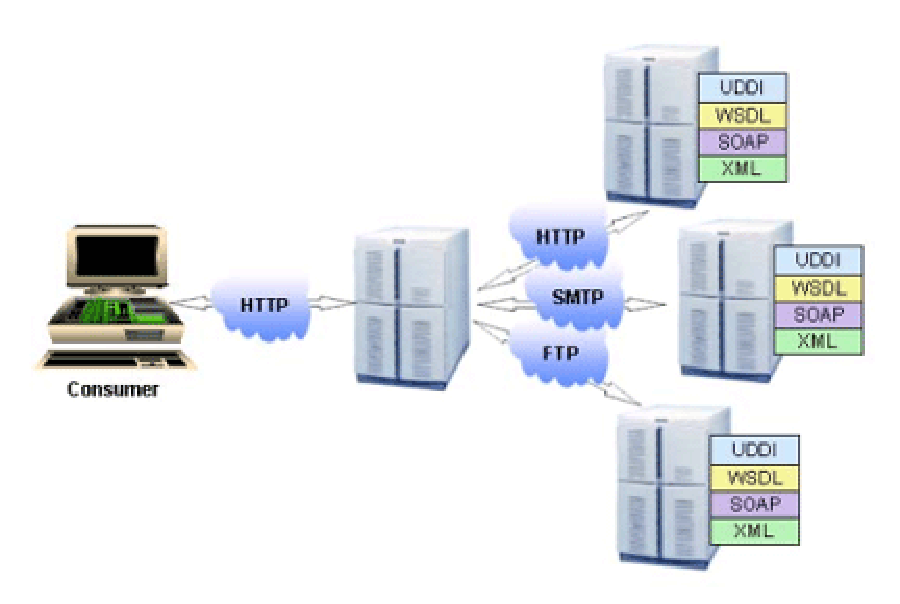
\includegraphics[width =\columnwidth]{Figures/clientserver.eps}
\end{center}
  \caption{Client-server web architecture}
  \label{arch}
\end{figure}

In this way, Service-Oriented Computing (SOC) paradigm promotes the use of services 
for the development of massively distributed applications, trying to achieve the creation of fast, 
low-cost, flexible and scalable applications \cite{Papazoglou2007}. 
Services are the main building block of this paradigm, being these services self-describing and platform-independent. 
Thanks to the use of standards for the description, publication, discovery and invocation, 
the services can be integrated without taking care of the low-level implementation 
details of each service. The aim of SOC is to make possible 
the creation of dynamic business processes and agile applications 
by providing an easy way to assemble application components into a loosely coupled network of services.

To reach the goals of SOC, a Service-Oriented Architecture (SOA) is defined. 
SOA is a software architecture based on the utilization of services, 
being these services provided to the user of the application or to other services in the network. 
This is possible by the use of service interfaces that can be published and discovered. 
SOA is based on a model of roles where every service can play multiple roles. 
For example, a service can offer certain functionality to a user and, at the same time, 
being the consumer of the functionality provided by some other services. 
Such model reduces the complexity of applications and increases their flexibility. 
Although at the beginning of SOA there were several architectures aspiring 
to become SOA standards \cite{Karp2000,Sun1999}, the most successful one was the architecture based on Web Services.

W3C defines a Web Service (WS) in the following way:

\begin{quotation}
	``A Web Service is a software system designed to support interoperable machine-to-machine interaction over a network. It has
an interface described in a machine-processable format (specifically WSDL). Other systems interact with the Web Service in a manner prescribed by its description using SOAP-messages, typically conveyed using HTTP with an XML serialization in conjunction with other Web-related standards.''
\end{quotation}

We can see in this definition that there are two basic standards 
related to Web Services: Web Service Description Language (WSDL) for the definition 
of the service functionality and its properties \cite{W3C2001}, 
and Simple Object Access Protocol (SOAP) for the exchange of 
XML messages between services \cite{W3C2007}. 
There is also an additional standard called Universal Description, Discovery and Integration (UDDI) 
used to create Web Service directories and to search for services 
in the network \cite{OASIS2004}, but this is a bit out of date. The use of these standard protocols is 
the key point to improve the integration between different parties in a web service architecture.

In Figure \ref{Figure1} a possible representation of the web service architecture stack is shown. 
One can see that the three standards described above are only a small part of the stack. 
One also need protocols to define security aspects (ensuring that exchanges of information 
are not modified or forgotten in a verifiable manner and that parties can be authenticated), 
to provide reliable messaging for the exchange of information between parties, 
to specify the collaboration between services when we compose them, 
to individually describe the behaviour of each service in a business process, etc. 
The problem is that whereas the standards for basic services (WSDL and SOAP) 
are widely adopted for their respective purposes, the situation is not very 
clear when we talk about composing services, 
having multiple protocols aspiring to become a standard in this layer.

\begin{figure}[h]
\begin{center}
\psfig{file=Figures/ws-stack.eps,scale=.55}
\end{center}
\caption{Web Service architecture stack.}
\label{Figure1}
\end{figure}

Two different approaches can be followed when we designing web service compositions. 
They are called \textit{orchestration} and \textit{choreography}. 
The former describes the individual business process followed by 
each one of the participants in the composition, 
while the latter describes the composition from a global viewpoint, 
defining the interactions (exchange of messages) happening between the parties, that is, 
how they collaborate in the composition. In Figure \ref{orch}, it is depicted graphically what it the role
of each of them if they are compared with the musicians in an orchestra. Despite these differences, the ideal solution would 
be fusing both approaches in a single language and environment \cite{Papazoglou2007}.

\begin{figure}[h]
\begin{center}
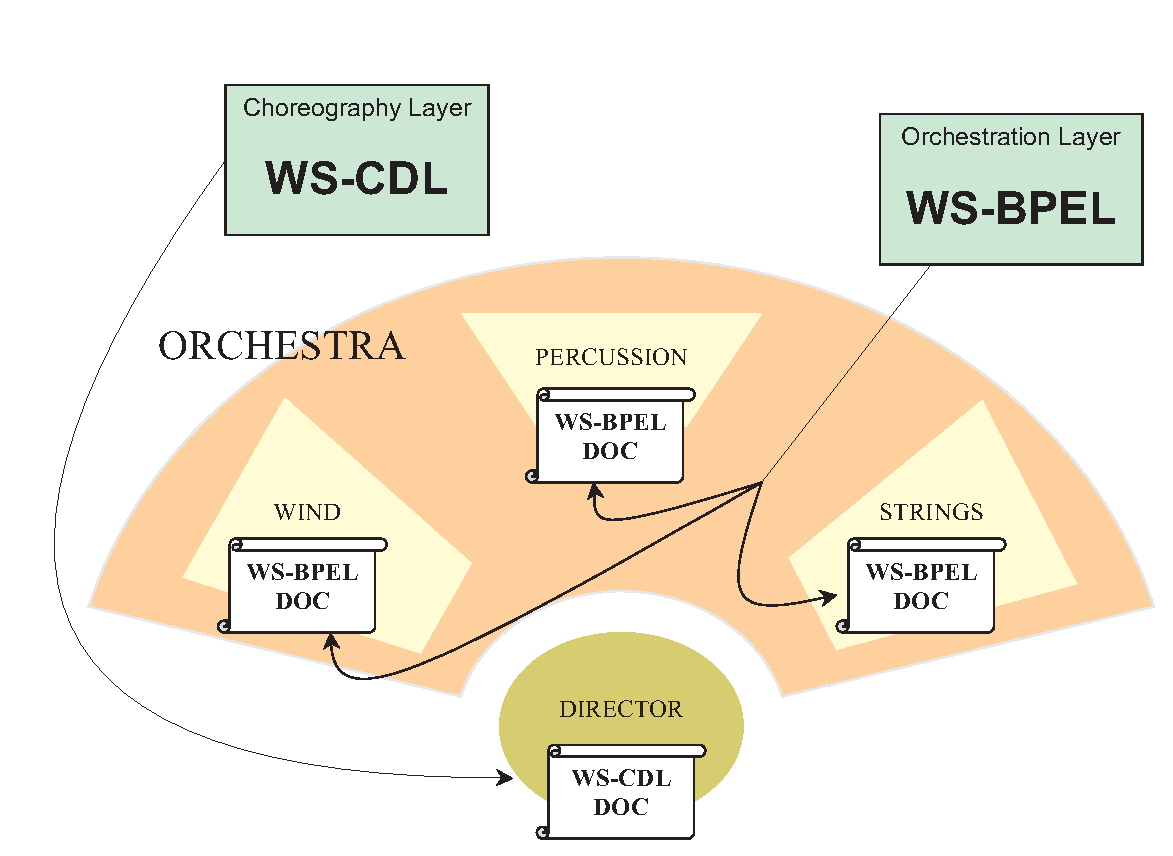
\psfig{file=Figures/orchestra.eps,scale=.5}
\end{center}
\caption{Choreography vs. Orchestration}
\label{orch}
\end{figure}

Anyway, the languages we can use in both cases should accomplish some common goals: 
(i) the capacity of modelling service interactions, including control flow and data constraints, 
(ii) the possibility of specifying exceptional behaviour, 
indicating which errors can happen in the execution of the composition 
and the way of handling these errors, and (iii) the ability to model web service compositions at a high level, 
without taking care of the implementation details of each one of the services.

{\bf Comment: Concluir ventajas y desventajas de cada uno.} 
Choreography on the other hand does not rely on a central coordinator. Rather, each
web service involved in the choreography knows exactly when to execute its operations
and whom to interact with. Choreography is a collaborative effort focused on exchange
of messages. All participants of the choreography need to be aware of the business
process, operations to execute, messages to exchange, and the timing of message
exchanges.
The most recent answer to the integration challenge is the Service Oriented
Architecture (SOA) and the web services technologies. The bottom-up view of the SOA
sees different business applications exposing their functionalities through web services.
Thus we can now access different functionalities of different legacy and new developed
applications in a standard way (through web services). Such access to functionalities is
important because typical companies have a large number of existing applications
which have to be integrated.
Regarding the choreography approach, there are several languages that 
have been designed for that purpose. One of the most popular languages 
is Web Services Choreography Description Language (WS-CDL), 
which specifies the common and complementary observable behaviour of 
all participants in a composition \cite{W3C2005}. 
It is based on XML and describes the peer-to-peer collaborations 
between the composite web services from a global point of view, that is, 
the exchange of messages to achieve a common business goal. 
The aim of this language is allowing the composition of any kind of web services, 
regardless of the platform hosting the service or the implementation language. 
Figure \ref{Figure2} is an example of how WS-CDL can be useful 
for the integration of different kinds of web services.

\begin{figure}[h]
\begin{center}
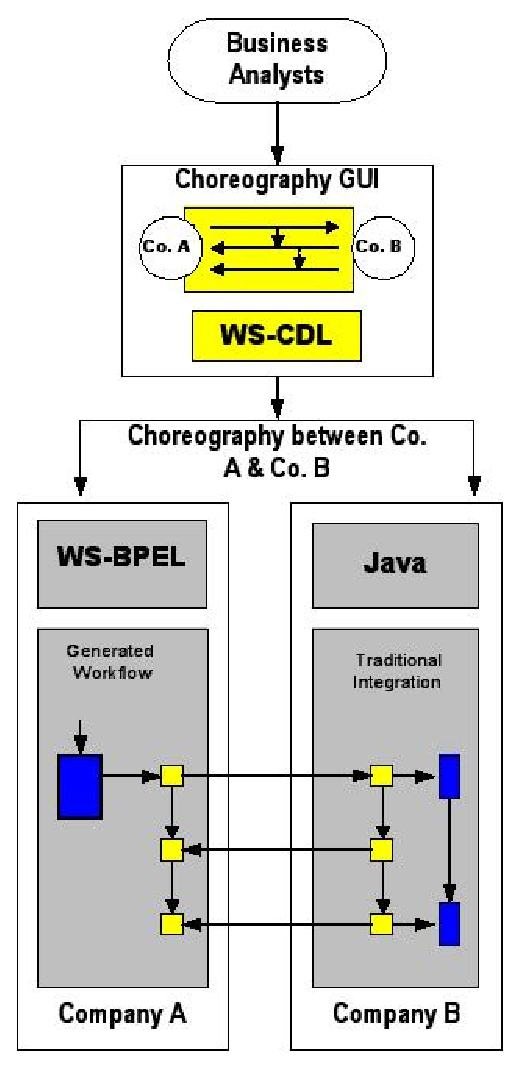
\psfig{file=Figures/WSCDL.eps,scale=.7}
\end{center}
\caption{Integration of Web Services using WS-CDL.}
\label{Figure2}
\end{figure}

A WS-CDL document defines a hierarchy of choreographies, where there is only one top-level choreography, marked explicitly as the \textit{root choreography}. The basic building block of a choreography is the \textit{interaction} element. It indicates information exchanges between participants, possibly including the synchronization of some information values. These interactions are performed when one participant sends a message to another participant in the choreography. When the message exchanges complete successfully, the interaction completes normally. 

We can distinguish two different kinds of \textit{complex activities} inside a choreography: the workunit element and the ordering structures. The \textit{workunit} element specifies a condition that must be fulfilled in order to perform some work and/or the repetition of some work. It completes successfully when the set of activities inside completes successfully. \textit{Ordering structures} are used to combine basic activities and other complex activities in a nested way, expressing the order in which actions are performed within the choreography. There are three ordering structures: The \textit{sequence} ordering structure expresses that the set of activities inside must be executed sequentially. The \textit{parallel} ordering structure indicates that the set of activities inside must be executed concurrently. It completes successfully when all the concurrent activities complete successfully. And the \textit{choice} ordering structure specifies that only one of multiple activities can be executed. If the choice have workunits inside, only the first one in lexical order with a ``true'' guard condition is selected. If there are other activities, there is no way to know which one is selected; it is considered as a non-observable decision.

Different types of exceptions are considered in WS-CDL. Exception workunits can be defined to handle all these exceptions. They may also be used as the mechanism to recover from the exceptions. At least one exception workunit must be defined. The guard of the workunit can be used to specify the particular type of exception we want to handle. Only one exception workunit can match each exception. If multiple exception workunits are defined, the order of evaluating them is based on the order in which the workunits have been defined. When the matching happens, the actions of the matched workunit are executed. If no matching happens and a default exception workunit exists, then the actions of this workunit are executed. Otherwise, the exception is raised in the parent choreography. WS-CDL also allows us to define finalization actions within a choreography that can confirm or cancel the effects of this choreography, so we can use this actions for compensation. 

Next, we introduce the orchestration approach used in this Thesis.

\subsection {WS-BPEL}
In 2002, researchers and engineers of the main companies of the world (IBM, Microsoft, etc.)
realised that the new and rapidly emerging process-oriented approach required the definition of 
a neat and precise language for describing how a set of intecting web services can be included
in a business process. Traditional methods for integration and business process automation 
typically involve embedded logic inside of applications designed 
to meet a specific business need such as ERP, supply chain, or CRM. 
The development, testing, and deployment efforts required 
to change these applications make integration and process changes both costly and complex \cite{}.
To address these issues, proprietary products emerged 
to abstract integration and process automation into a new layer of software tools. 
These software products liberated integration and process tasks from 
the underlying business systems so they could be more effectively changed, managed, and optimized.
The idea and motivation behind almost each new technology and platform for
enterprise application development is to provide an environment where better
business applications can be developed with less effort and these business applications
should closely align to the business processes, which should not be too complex, and
which can be adapted to the changing nature of business processes without too much
effort. Within companies, business applications have to
interoperate and integrate. Integrating different
applications has always been a difficult task for various functional and technology
related reasons \cite{}.

The Business Process Execution Language for Web Services (BPEL4WS), for short BPEL, 
was first conceived in July, 2002 with the release of the BPEL4WS 
1.0 specification. This first draft was initially developed by just three companies, IBM, Microsoft, and BEA. 
This document proposed an orchestration language inspired 
by previous variations such as Web Services Flow Language (WSFL), developed by IBM and XLANG specification language developed
by Microsoft. WSFL was designed by IBM and is based on the concept of directed graphs.
XLANG was designed by Microsoft and is a block-structured language. BPEL combines
both approaches and provides a rich vocabulary for description of business processes. After this first attempt, other major companies such as SAP and Siebel Systems joined the former ones to write
the version 1.1 of the BPEL4WS specification that was released less than a year later, in May of 2003. 
Fortunately, this brand new version received much more attention and vendor support, 
leading to a number of commercially available BPEL4WS-compliant 
orchestration engines \cite{}. Before publishing this release, 
the BPEL4WS specification was submitted to an OASIS 
technical committee in order to be evaluated so that the specification could be developed into an official and open standard.
This technical committee was active from April 2003 to May 2007, 
and, during this time, a lot of contributions and improvements were received. 
In April 2007, WS-BPEL version 2.0 was approved as an OASIS standard. 
As a proof of maturity, more than 37 organizations collaborated to develop WS-BPEL, including representatives of Active Endpoints, Adobe Systems, BEA Systems, Booz Allen Hamilton, EDS, HP, Hitachi, IBM, IONA, Microsoft, NEC, Nortel, Oracle, Red Hat, Rogue Wave, SAP, Sun Microsystems, TIBCO, webMethods, and other members of OASIS \cite{}.
Finally, in January 2008, another OASIS technical committee started 
to define a WS-BPEL extension to emcompass the definition of 
human interactions (``human tasks'') as part of a WS-BPEL process. Figure \ref{bpelevolution} summarises this evolution-

\begin{figure}[h]
\begin{center}
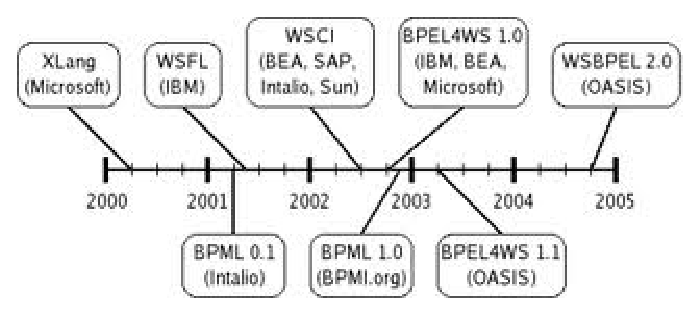
\psfig{file=Figures/bpelhistory.eps,scale=.7}
\end{center}
\caption{WS-BPEL evolution.}
\label{bpelevolution}
\end{figure}

Moreover, there were established ten original design goals associated with the definition of WS-BPEL \cite{wsbpelstandard}:
\begin{itemize}
\item Define business processes that interact with external entities 
through web service operations defined using WSDL, and that 
manifest themselves as web services defined using WSDL. 
\item Define business processes using an XML-based language. 
Do not define a graphical representation of processes or provide any particular design methodology for processes.
\item Define a set of web service orchestration concepts that are meant to be used by both the external (abstract) and internal (executable) views of a business process. Such a business process defines the behavior of a single autonomous entity, typically operating in interaction with other similar peer entities. 
%It is recognized that each usage pattern (i.e., abstract view and executable view) will require a few specialized extensions, but these extensions are to be kept to a minimum and tested against requirements such as import/export and conformance checking that link the two usage patterns.
\item Provide both hierarchical and graph-like control regimes, and allow their use to be blended as seamlessly as possible. This should reduce the fragmentation of the process modeling space.
\item Provide data manipulation functions for the simple manipulation of data needed to define process data and control flow.
\item Support an identification mechanism for process instances that allows the definition of instance identifiers at the application message level. Instance identifiers should be defined by partners and may change.
\item Support the implicit creation and termination of process instances as the basic lifecycle mechanism. Advanced lifecycle operations such as ``suspend'' and ``resume'' may be added in future releases for enhanced lifecycle management.
\item Define a long-running transaction model that is based on proven techniques like compensation actions and scoping to support failure recovery for parts of long-running business processes.
\item Use Web Services as the model for process decomposition and assembly.
\item  Build on Web services standards (approved and proposed) as much as possible in a composable and modular manner.
\end{itemize}

As a result, WS-BPEL along with web services technologies provide now a standardized integration interface 
and a standardized language for the integration of different services as well as for the automation of some tasks. 
Nevertheless, web scenarios are becoming more and more complex since they highly heterogeneous, that is, a lot of different
services from different companies interact jointly to perfom a particular task. In particular, it is known
that business processes change relatively often due to this heterogeneity. Therefore, designers 
do not need only a way to compose a set of services, rather they also
need a way to compose and modify them in the right order and in a relatively 
uncomplicated and straightforward way. Due to this, BPEL is sometimes compared 
to general purpose programming language, but it
is not as powerful as one of the well-known programming language \cite{}. However, 
it is simpler and better suited for business
process definition and, therefore, BPEL must be considered a supplement to
modern languages rather a replacement.

%The first version of BPEL has been developed in August 2002 by BEA, IBM, and
%Microsoft. Since then the majority of vendors have joined which has resulted in several
%modifications and improvements and adoption of version 1.1 in March 2003. In April
%2003, BPEL was submitted to OASIS (Organization for the Advancement of Structured
%Information Standards) for standardization purposes where the WSBPEL TC (Web
%Services Business Process Execution Language Technical Committee) has been formed
%since. This
%has led to even broader acceptance in industry.


%there are two possible ways to compose a set Choreography has not gained support from the
%industry which would be comparable to BPEL \cite{}.
%This is where the BPEL (Business Process Execution Language for Web Services, also
%WS-BPEL or BPEL4WS) becomes important. BPEL allows composition of web services
%and is thus the top-down approach to SOA ? the process oriented approach to SOA.
%Let us have a closer look at a typical BPEL process. First, the BPEL business process
%receives a request. To fulfill it, the process then invokes the involved web services and
%finally responds to the original caller. Because the BPEL process communicates with
%other web services, it relies heavily on the WSDL description of the web services
%invoked by the composite web service.

After briefly introduce its history and design goals, we discuss next its technical details. 
BPEL is therefore an orchestration
language in the sense that it is used to define the composition
of services from a local viewpoint, describing the individual
behaviour of each participant. Choreography is covered by other standards,
such as WS-CDL (commented previously). BPEL is designed to support the description of both behavioural service interfaces and executable
service-based processes \cite{OuyangVABDH07}. A behavioural interface (known as abstract process) is a specification of the
behaviour of a class of services, capturing constraints on the ordering of messages to be sent to and
received from a service. An executable process defines the execution
order of a set of activities (mostly communication activities), the partners involved in the process, the
messages exchanged between partners, and the events and exception handling specifying the behaviour
when specific events or faults occur. In Figure \ref{bpelexample}, we can observe an example of the typical business process
of a travel agency.

\begin{figure}[h]
\begin{center}
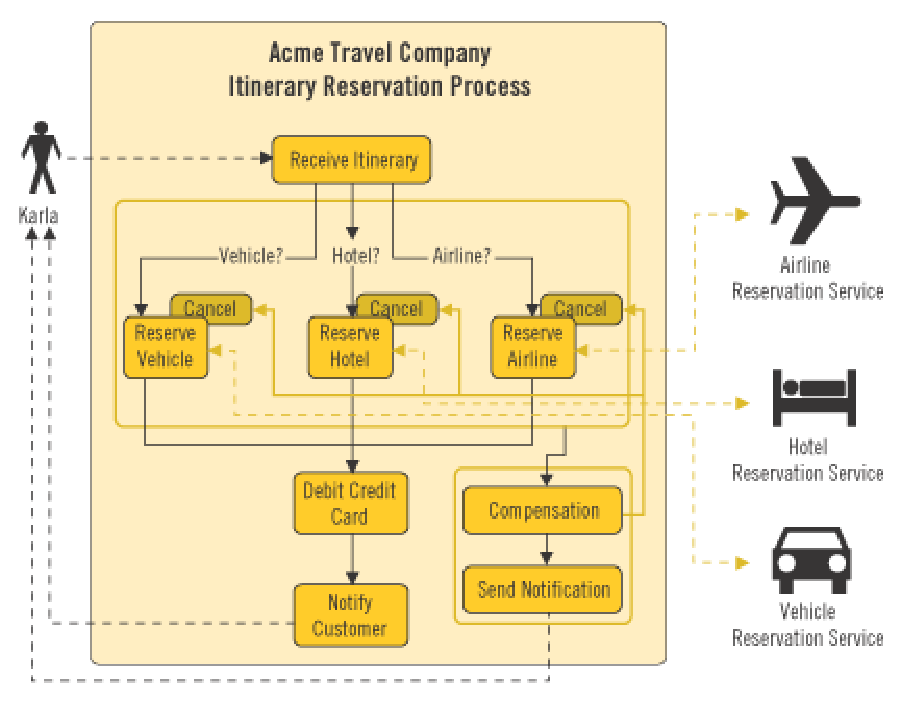
\psfig{file=Figures/bpelexample.eps,scale=.7}
\end{center}
\caption{Example of a business process workflow.}
\label{bpelexample}
\end{figure}

According to the standard of WS-BPEL, an  abstract process is a partially specified process that is not intended to be executed
and it must be explicitly declared as ``abstract''. As its name indicates, 
an abstract process may hide some of the required 
operational details expressed by an executable artifact.
All the constructs of executables processes are made available to abstract processes
and, consequently, they share the same expressive power \cite{}. 
Therefore, the main different between an abstract and a executable processes is 
that the second one contains the exact details of business processes and, consquently,
it is intended to be executed in an orchestration engine, whereas the first one serve a descriptive role,
defining the message exchange between the parties involved. Specifically, an abstract process is usually use to 
describe the observable behavior of some or all of the services offered by an
executable process and/or to define a process template that contains domain-specific best practices. 
Such a template can be seen as a design-time representation of the process logic, excluding execution details to be
completed when mapping to an executable process.
In most cases BPEL is used for
executable processes \cite{}.
Moreover, the definition of conceptual model in which one can define an abstract or an executable
process is a key feature of WS-BPEL since the processes execute and interact with their
partners in a consistent way regardless of the supporting platform or programming model used
by the implementation of the hosting environment, unlocking the potential of
web services because it allows the development of tools and other technologies that greatly
increase the level of automation and thereby lower the cost in establishing cross enterprise
automated business processes. In addition to this, abstract process ensures the level of privacy required by the 
companies since the implementation of the service is hidden to the other participants. 

In detail, WS-BPEL is an XML-based language which
supports the web services technology stack, including SOAP, WSDL, UDDI and so on. 
It defines a model and a grammar for describing the behavior of a business process
based on interactions between the process and its partners as well as the order of these interactions. 
The interaction with each partner is performed through web service interfaces, 
and the structure of the relationship at the interface level
is encapsulated in what is called a partnerLink. WS-BPEL also introduces 
mechanisms for dealing with business exceptions and faults. Moreover, WS-BPEL
introduces a mechanism to define how activities have to be compensated in cases 
where exceptions occur or a partner requests reversal.
A WS-BPEL process is a reusable definition that can be deployed in different ways and in
different scenarios, while maintaining a uniform application-level behavior across all of them.


\begin{figure}[h]
\begin{center}
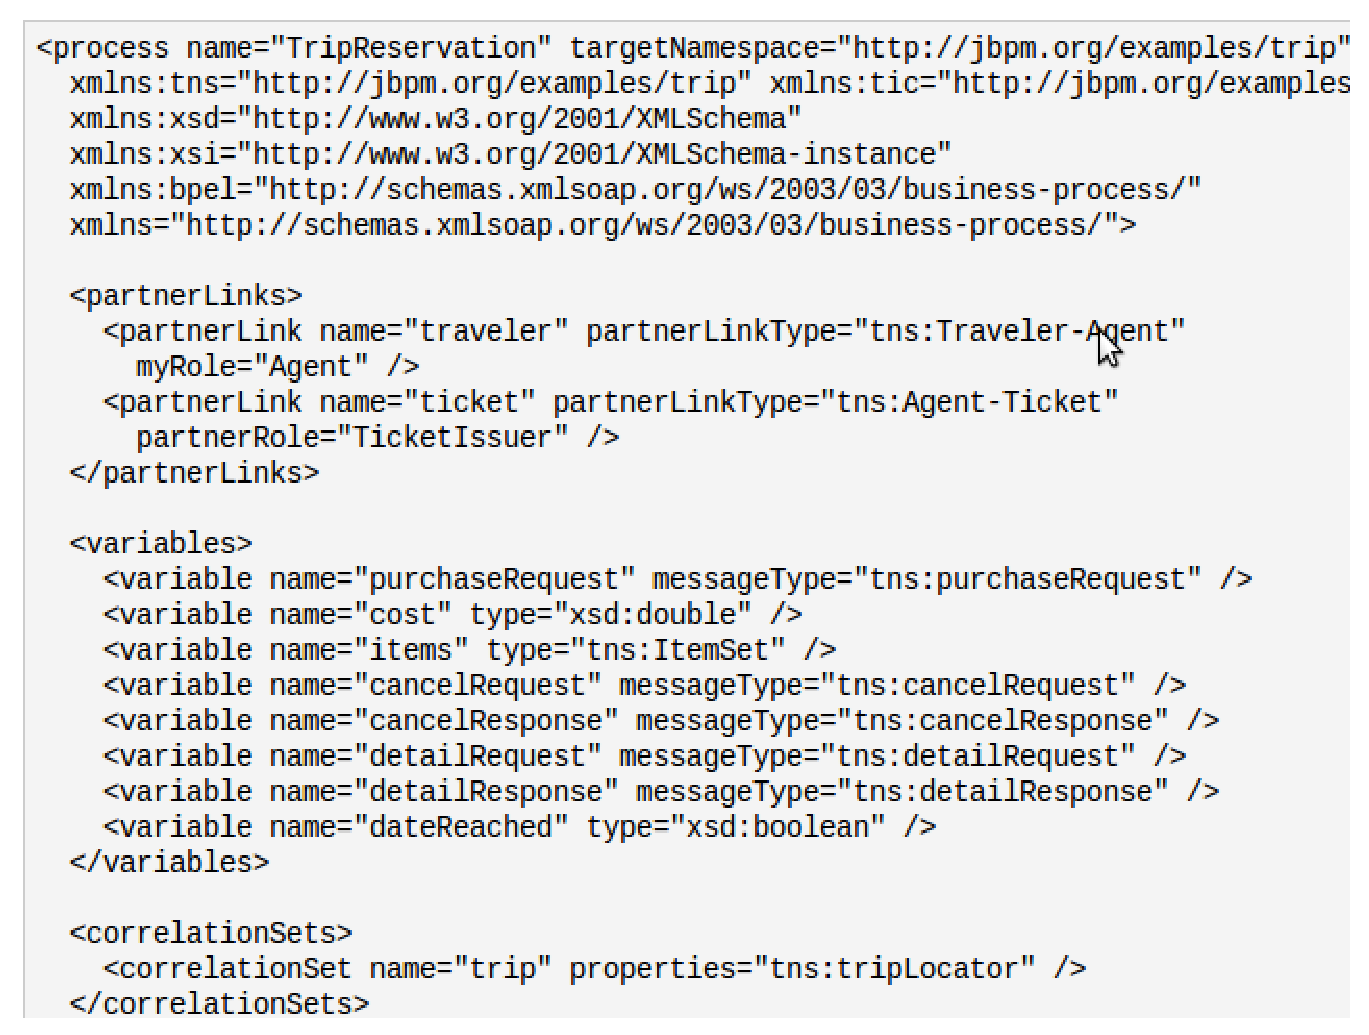
\psfig{file=Figures/bpelcode.eps,scale=.5}
\end{center}
\caption{WS-BPEL code.}
\label{bpelcode}
\end{figure}

In Figure \ref{bpelcode}, we can observe a piece of the BPEL code for a booking process. 
BPEL processes use {\em variables} to temporarily store 
data. Variables are therefore declared on a process or on a scope 
within that process. Also, 
it provides \emph{basic} or \emph{structured} to declare the process logic. 
\emph{Basic activities} are those which describe the elemental 
steps of the process behaviour \cite{}: 
\begin{itemize}
\item The activity \emph{assign} is used to assign data to the variables defined in the process. 
This activity can be used to copy data from one variable to another as well as to
populate new data in a variable using expressions. As usual, expressions are constructed using 
variables and constants. 
\item The activity \emph{empty} is devoted to be used as an activity that does nothing. For instance, one can
decide to capture an exception and do nothing to handle it. Another use of \emph{empty} is
to provide a synchronization point in a parallel activity.
\item The activity \emph{wait} specifies a particular delay or deadline. 
\item To invoke a web service of service provider, WS-BPEL offers the activity {\em invoke}. 
Normally, this activity is used to request an operation in a service. This operation is usually 
a basic activity in the provider. Operations can be of two types: request-response or one-way.
One-way consist of sending a message (some variables can be enclosed) so that no response is expected
as part of the operation, whereas a request-response invocation requires a message back. Evidently, this
response message can be used to notify the sender about a fault during the operation. A more detailed
explanation will be provided in Chapter \ref{chapter:c3}. 
\item A \emph{receive} activity is necesary to receive the message sent in the invoke activity.
messages, the portType (optional) and operation that it expects the partner to invoke. The
value of the partnerRole in the partnerLink is not used when processing a <receive> activity.
In addition, it specifies a variable, using the variable attribute, to
store the message the operation to be requested. In many cases, this activity is the first part of the process.
\item The \emph{reply} activity is used to respond to a request previously accepted through an
inbound message activity. For instance, it can be used in conjunction with the receive activity
to respond to the invocation of a service. Clearly, it is only meaningful
for request-response interactions, but a one-way ``response'' can be sent by invoking the
corresponding one-way operation on the sender. Finally, it may specify a
variable attribute that references the variable that contains the message data to be sent.
\item The activity \emph{throw} is used to signal an internal fault explicitly.
\item The activity \emph{exit} is used to immediately end the process instance.
\item WS-BPEL provides the user with the ability to declare new activities that are
not contemplated in the specification. This is done using the \emph{extension activities}. This
extension is not explicitly contemplated in the theory of this Thesis, although they are required
to implement the theory in an orchestration engine.
\item Finally, using the activity \emph{rethrow} in a fault handler, it is possible to rethrow a fault.
For instance, this activity is useful when the situation that causes the fault is not solved after
the completion of the fault handler and, therefore, it is needed to redo this handler to check if the
situation has been solved afterwards.
\end{itemize}  

On the other hand, \emph{Structured activities} encode the control-flow logic of the process.
The set of structured activities defined in the standard are the following:
\begin{itemize}
\item The activity \emph{sequence} includes a set of activities that are performed sequentially in the
order in which they appear in the structure. It ends
when the last activity in the sequence has finished.
\item The activity \emph{flow} provides concurrency and synchronization, creating 
a set of concurrent activities directly nested within the process and it enables
synchronization dependencies between activities that are nested to it. A more detailed explanation
of how this activity works is given in Chapter \ref{chapter:c3}.
\item The activity \emph{if} specifies conditional behavior. As usual, the activity consists of an ordered list of one or
more conditional branches defined by the ``if'' and optional ``elseif'' elements, followed by an
optional ``else'' element.
\item The activity \emph{while} provides conditional repetitive behaviour.
\item \emph{RepeatUntil} provides the repeated execution of a contained activity. The difference with
the activity while is that the inner activity is executed at least once.
\item The activity \emph{pick} waits for the occurrence of exactly one event from a set of events, and then
executes the activity associated with that event. After an event has been selected, the other events
are no longer accepted by that ``pick''. Moreover, a deadline for the occurrence of such events can be established
in such a way if this deadline experies the pick activity ends. This structure has some similarity the choice operator in
a process algebra althoudh with a predefined timeout. 
In WS-BPEL, it can be compared with a set of receive activities that run in parallel, where just only one can be executed,
and a common deadline for the execution of these receive activities is set (to this end, the wait activity can be used).
\item Lastly, the standard offeres an activity (forEach) to execute the contained activity a predefined number of times that
is expressed in the definition of the activity.
\end{itemize}


\section{Heterogeneous Distributed Systems: Grid/Cloud Computing}

In 1943, the president of IBM, Thomas J. Watson, predicted:

\begin{center}
``I think there is a world market for about five computers''
\end{center}

In recent times, this phrase has been widely discussed since some authors
consider that it is an clear example of failed prediction. Nevertheless, with the advent of new computational 
such as Grid and Cloud Computing, some authors argue that it will become a reality soon. In addition,
other authors consider that this phrase is completely true nowadays since there five big companies that
are monopolising the world market \cite{}.

Thanks to the fast development of society, daily basic services such as water, electricity, gas and telephone services 
are commonly supplied to citizens so that everybody can have 
immediate access to them in developed countries. Today, these services 
known as ``utility'' services since customers are charged according to the consumption. In 1969, Leonard Kleinrock, one of the leading scientists of the American ARPANET agency, said: ``Today, computer networks are in their infancy, but as they grow and become more sophisticated we will see the rise of the \emph { Utility computing}. It is amazing how in 1969 a scientist could already see the usefulness of computers and the advent of a distributed computing model that would be based on providing services and paying for them. What makes this statement more fascinating is that this year is when the Internet was born. The first version only connected 2 computers worldwide, but this person was already thinking that someday the Internet could connect millions of computers into a single network. This vision of computing (based on a model of on demand service provisioning) anticipated the massive transformation of the computer industry in the XXI century. 

Thus, major companies such as Google, Amazon or Microsoft are introducing it in their business model. Moreover, it
is often confused with Cloud and Grid Computing. Utility Computing 
is the underlying business model for a Grid or Cloud infrastructure, i.e. it
can be seen as a mean of charging customers  for computing services so that 
users pay only for the consumption, whereas the costs associated with the production and distribution of computing services 
will be undertaken by the provider. As happens with revolutionary software, 
protocols or any computer-related paradigm, Cloud Computing must undergo 
a series of steps to check if all benefits 
that providers are promising really serves companies to save costs and enhance the competitiveness. 
In this sense, Larry Ellison, founder and CEO of Oracle, believe that Cloud Computing 
is nothing more than a new way of naming what companies have been doing so far \cite{abovetheclouds}: 
\begin{quote}
``The interesting thing about Cloud Computing is that we have redefined Cloud Computing 
to include everything that we already do\ldots I do not understand what we would do differently in the light of Cloud
Computing other than change the wording of some of our ads.''
\hspace{5cm}\emph{Larry Ellison, quoted in the Wall Street Journal, September 26, 2008.}
\end{quote}
Many researchers have tried to define the term ``Cloud Computing'' without reaching 
a standard definition. For instance, Buyya et al. \cite{} define a cloud system as:
\begin{quote}
``A cloud is a parallel and distributed system consisting of a collection of 
virtualized and interconnected computers that have been provisioned dynamically 
and they are presented as a single computational resource based on service level agreements (SLAs) 
established by negotiation between the service provider and the consumer.''
\end{quote} 

In \cite{vaq09} one can find up to 21 different definitions of Cloud computing. For instance, Luis M. Vaquero et al. defines the Cloud as:
\begin{center}
\emph{``The Cloud is a large and easy to use container of virtualized resources 
(such as hardware, services, development platforms \ldots). These resources can be 
dynamically reconfigured to fit into a variable load (scale), allowing also the optimal use of these resources. 
This service is exploited through pay-per-use model that is guaranteed by agreements.''}
\end{center} 

{\bf Meter un par de p�rrafos de Grid}

Finally, the main difference between a Cloud-oriented and a Grid-oriented system relies in the virtualisation of resources. 
In a Grid infrastructure, users do not share in real-time the resources allocated to them, 
whereas in a Cloud infrastructure the virtualisation is essential to serve more users,
thus getting the savings promised by suppliers \cite{}.

\section{Web services vs. Grid/Cloud Computing}

In this section it is presented a summary of the main differencies and sinergies between web services and
Grid/Cloud Computing since a formal language to mix both approaches is one of the parts of this
Thesis. First, one can consider that web services are themselves software offered as a service (SaaS)
and a system can be seen as a composition of services communicated via the Internet
that coordinate to perform a certain task. Nevertheless, 
there are still some differences between both approaches such as standardization. Above,
we presented two (WS-CDL and WS-BPEL) of the standards to model web services compositions, but
it is impossible to present a standard that describes the main concepts of Cloud Computing and, to some
extent, of Grid Computing. One of the reasons is that Cloud and Grid are relatively new and, therefore,
there has not been time to agree a standard for them. The other reason is related to commercial policies since
many big companies are competing to impose its services.  
So far, there is nothing new, but the main difference lies in virtualization, 
since different services provided by the cloud are performed in virtual 
machines rather than directly on a server such as the case of a web service, 
and, therefore, the concurrency in the system is higher. 

Another difference is data persistence. Web services are usually ``stateless'', which means that
no state is saved in the system after performing a operation invoked in the service. The only way to save
the state of this operation is to store it in a database. The main disadvantage of this approach is that there is no
standardization and, therefore, this operation is platform dependent and it will depend of the application scope. 
In this Thesis, we use a standard called Web Services Resources Framework (WSRF) that it is intended to solve this problem. 
The main advantage of it is that all the steps are standardised so that the cooperation 
between such systems is simple. Another advantage is that the user can decide which 
resources can take part in the interaction. WSRF is described in the next section. 

In addition, Cloud/Grid computing could be considered as a layer to be placed on the bottom of the web services, 
and use them as a mean to access the resources. Thus, new standards must be defined in a similar fashion as in
WSRF, but taking into account the particularities of the Cloud infrastructure. Here, we must emphasise that Cloud 
Computing is not only to provide software as a service, but there are infrastructure and platform as a service, 
which web services cannot cover. 



\section{Web Services Resource Framework}

The aim of this section is to introduce the basic concepts for the management 
and destruction of stateful web services, i.e., web services with 
a set of resources associated to store the
state after ending an operation. In this sense, we call \emph{WS-Resource} 
to the association between a web service and a persistent resource.
To manage stateful web services, it is required to 
define the patterns used to create the relationship between the service and the resource. These patterns
will reuse in most of the cases a series of widely studied technologies, e.g. WS-Addressing. 
Moreover, it is need to define how the properties of the resources can be accessible 
from outside. This is usually done through an interface.

The architecture provided by web services has been widely accepted as a means of 
structuring the interactions between services that are part of a distributed system 
and work together to achieve a common goal. Currently, developers require a higher 
degree of standardization to provide additional interoperability between such services, 
but until mid-2004 no research group or group of experts had seriously considered the idea of 
proposing a standard for modelling the communication between stateful services, that is, services
endowed with an associated persistent resource. 
Thus, in January of 2004, several members of the organization Globus Alliance and the multinational IBM 
defined, with the help of experts from companies such as HP, SAP, Akamai, etc., 
the first specification and the basis of an initial architecture. 
In March of 2004, these documents were sent to the organization responsible for the standardization, 
OASIS. Initially, two committees were formed to study and develop 
certain parts of the recently created standard. 
On the one hand, it was created the \emph{WSRF Technical Committee}, which worked on four specifications:
\emph{WS-ResourceProperties, WS-ResourceLifetime, WS-Servicegroup}, 
and \emph{WS-BaseFaults}. Moreover, the \emph{WSN Technical Committee} 
was responsible for the rest of the specifications: \emph{WS-BaseNotification, WS-Topics}, and \emph{WS-BrokeredNotification}.

WS-Resource Framework is inspired by the work previously done by Global Grid Forum's 
Open Grid Services Infrastructure (OGSI) Working Group \cite{Foster03}. More specifically,
WSRF can be seen as a simple refactoring of concepts and interfaces 
developed in the specification \emph{OGSI V1.0},
exploiting recent developments in the area of web services (e.g. WS-Addressing). 
WS- Resource Framework \cite{BAN06} is a specification, whose purpose is to define a 
generic framework for modelling and accessing WS-Resources and the relationships 
between them in a Grid/Cloud environment. In detail, WSRF defines 
the representation of the WS-Resource, specifying the messages exchanged and 
the XML documents required to manage the resource. 
A WS-Resource is defined as (i) the combination of an XML document with a type defined
by one or more \emph{portTypes} (a service may play different roles in the same interaction) and (ii) it must 
be addressed and accessed according to implied resource pattern. This pattern is a derivation 
of the \emph{Endpoint References} included in the standard WS-Addressing. 
WS-Addressing is used to standardise the endpoint reference of a WS-Resource. This endpoint
reference is the address of the WS-Resource at
a given network endpoint and it must be used to identify the resource in any exchange of messages. 

Typically, web service interfaces provide users with the ability to access and manipulate its state, e.g. data values
that evolve by the interaction among various services. In other words, 
the message exchanges that are implemented in the behavior of the services 
are intended to allow persistent access to these resources. However, this notion is not 
as evident in the definition of the interface \cite{Fost04}. The messages sent and received 
by these services involve (or encourage the programmer to infer) the existence of an resource. 
Therefore, it is desirable the definition of standards that allow the discovery, 
creation, manipulation and destruction of these resources. These standards should make this 
complex environment as interoperable as possible. Furthermore, 
WSRF offers mechanisms to declare, access, monitor and destroy WS-Resources by using conventional techniques, 
which makes it easy to run in any platform since it is not necessary to take into account the decision logic of the resource owner.
It also includes mechanisms to describe how to check the status of a resource 
and how to make it accessible through its interface (described in WSDL). 
In detail, WSRF includes the mechanisms defining the means by which \cite{}:

\begin{itemize}
\item a WS-Resource can be destroyed, either synchronously attending to a
destroy request or a time-based (scheduled)
destruction, and specified resource properties may be used to inspect and monitor the lifetime of a WS-Resource (WS-ResourceLifetime);
\item the state of  a WS-Resource 
can be queried and modified via Web services
message exchanges (using the specification WS-ResourceProperties);
\item an endpoint reference (WS-Addressing) can be renewed in the
event the information contained becomes invalid
or stale (WS-RenewableReferences);
\item a collection of heterogeneous of web services can be defined,
whether or not the services are WS-Resources (WS-ServiceGroups); and 
\item fault reporting can be made more standardized through use of predefined XML
template (WS-BaseFaults). 
\end{itemize} 

\subsection{WS-ResourceProperties}

As mentioned above, WSRF uses a particular specification 
for defining the properties (attributes) of a WS-Resource, which is composed of 
the definition of the interface in WSDL and an XML ocument (Resource Properties Document) 
that specifies its properties. For example, these properties can be the disk size, processor capacity, etc.
As usual, there is a number of messages in the specification to update one or more of theses properties or to retrieve this
information. 

From now on, we suppose that the Resource Properties Document is:

\lstset{language=XML, numbersep=5pt,basicstyle=\small, frame=single}
\begin{lstlisting}
...
<GenericDiskDriveProperties 
xmlns: tns=``http://example.com/diskDrive'' >
  <tns:NumberOfBlocks>22</tns:NumberOfBlocks>
  <tns:BlockSize>1024</tns:BlockSize>
  <tns:Manufacturer>DrivesRUs</tns:Manufacturer>
</GenericDiskDriveProperties>
...
\end{lstlisting}

In WSRF, the operations that can be done are:

\begin{description}
\item[GetResourceProperty]
As the name suggests, this operation allows services to request 
the value of only one property of the document.

For instance, a possible request can be:

\lstset{language=XML, numbersep=5pt,basicstyle=\small, frame=single}
\begin{lstlisting}
...
<s12:Body>
  <wsrp:GetResourceProperty 
    xmlns:tns=``http://example.com/diskDrive''>
     tns:NumberOfBlocks
  </wsrp: GetResourceProperty>
</s12:Body>...
\end{lstlisting}

\item[GetMultipleResourceProperties]
This method is equivalent to the last one, but it is intended to retrieve
more than one property of the document at the same time. 
It can be used to prevent network congestion. The message would be:

\lstset{language=XML, numbersep=5pt,basicstyle=\footnotesize ,frame=single}
\begin{lstlisting}
...
<wsrp:GetMultipleResourceProperties
 xmlns:tns=``http://example.com/diskdrive''>
 <wsrp:ResourceProperty>tns:NumberOfBlock</wsrp:ResourceProperty>
 <wsrp:ResourceProperty>tns:BlockSize</wsrp:ResourceProperty>
</wsrp:GetMultipleResourceProperties>
...
\end{lstlisting}

\item[SetResourceProperties]
This specification allows to change some properties in the document. There are three kind of changes:

\begin{itemize}
\item Insert: It allows to add new properties to the document.
\item Update: It is used to update the value of a property.
\item Delete: To delete a property from the document.
\end{itemize}

A possible request can have the following form:

\lstset{language=XML, numbersep=5pt, basicstyle=\small,frame=single}
\begin{lstlisting}
...
<s12:Body>
 <wsrpw:SetResourceProperties
        xmlns:tns=``http://example.com/diskdrive''>
   <wsrp:Update>
    <tns:NumberOfBlocks>143</tns:NumberOfBlocks>
   </wsrp:Update>

   <wsrp:Delete resourceProperty=``tns:Manufacturer''/>

   <wsrp:Insert>
    <tns:someElement>42</tns:someElement>
   </wsrp:Insert>

 </wsrp:SetResourceProperties>
</s12:Body>
...
\end{lstlisting}

As it can be observed, it is possible to concate more than one operation in the same request. 
After proccesing this request, the document must look like this:

\lstset{language=XML, numbersep=5pt, frame=single}
\begin{lstlisting}
...
<GenericDiskDriveProperties
  xmlns:tns=``http://example.com/diskDrive''>
  
  <tns:NumberOfBlocks>143</tns:NumberOfBlocks>
  <tns:BlockSize>1024</tns:BlockSize>
  <tns:someElement>42</tns:someElement>

</GenericDiskDriveProperties>
...
\end{lstlisting}

\item[QueryResourceProperties]
This method is used for querying resource properties. 
For example, if one wants to know if the number of blocks is greater than 20 and the block size is 1024,
the following query gets this information:

\lstset{language=XML, numbersep=5pt, frame=single}
\begin{lstlisting}
...
<s12:Body>
 <wsrp:QueryResourceProperties>
  <wsrp:QueryExpression
   Dialect=``http://www.w3.org/REC-xpath-19991116''>
    boolean(/*/NumberOfBlocks>20 and /*/BlockSize=1024)
  </wsrp:QueryExpression>
 </wsrp:QueryResourceProperties>
</s12:Body>
...
\end{lstlisting}

The response must look like this:

\lstset{language=XML, numbersep=5pt, frame=single}
\begin{lstlisting}
...
<s12:Body>
 <wsrp:QueryResourcePropertiesResponse>
   true
 </wsrp:QueryResourcePropertiesResponse>
</s12:Body>
...
\end{lstlisting}

\end{description}

\subsection{WS-Base Faults}
Normally, a designer uses web service interfaces defined by others, and, therefore,
a method to standardize the format of error messages would facilitate the work of developers. 
This is the goal of WS-BaseFaults, where an error message has the following format:

\lstset{language=XML, numbersep=5pt, frame=single}
\begin{lstlisting}
...
<BaseFault> 
  <Timestamp>xsd:dateTime</Timestamp> 
  <OriginatorReference> 
    wsa:EndpointReferenceType 
  </OriginatorReference> ? 
  <ErrorCode dialect=``anyURI''>xsd:string</ErrorCode>? 
  <Description>xsd:string</Description> * 
  <FaultCause>wsbf:BaseFault</FaultCause> * 
</BaseFault>
...
\end{lstlisting}
where:

\begin{itemize}
\item Timestamp: It is the exact instant where the error happened.
\item OriginatorReference: This is the endpoint reference of the service that originated the error.
\item ErrorCode: Error code (e.g. POSIX errno) to be used by error handling systems .
\item Description: Explanation of the cause of error (in natural language).
\item FaultCause: Technical cause of the error. 
\end{itemize}
Finally, note that it is possible to report an error whithout using this format, but WSRF provides it
to help participants to manage it in a consistent way.
\subsection{WS-ServiceGroup}
This specification allows users to create groups of services 
that share a number of properties in common, i.e., it is useful to group different web services that have similar behaviours.

\subsection{WS-ResourceLifetime}
The lifetime of a WS-Resource is defined as the period between its instantiation and its destruction. 
The goal of this specification is to standardise the process of destruction of a 
resource and define mechanisms to monitor its lifecycle. Surprisingly, the proces to create the WS-Resource
is not specified. The reason is that WSRF is intended to be used in the interaction and, therefore, the 
internal details of each participant are hidden. Thus, this specification meets the requirements of SOC
architecture presented previously and the transition from service-oriented architecture to resource-oriented
architecture is small. For technical reasons, we have included in our language
BPELRF a primitive to create the resource. 

Generally, in distributed systems, clients just want to use a resource for a given time interval.
For instance, in subscription systems, users decide normally the duration of the subscription.
Nevertheless, in many scenarios is most appropriate to provide a manner to immediately destroy 
the resource. Following the same example, it could happen that the client wants to interrupt its subscription 
and hence the immediate destruction must be provided. 
As discussed above, WSRF gives two ways to destroy a 
WS-Resource: immediate or scheduled.

\begin{description}
\item[Immediate destruction] To activate this kind of destruction, it is only required to add the attribute
\emph{$<wsrl:Destroy/>$} inside the field ($<Body>$) of the SOAP message that will be sent to the service
To confirm the destruction, the receiver must send the same message including the attribute
\emph{$<wsrl:DestroyResponse/>$} in the field (\emph{$<Body>$}) of the response SOAP message.

\item[Scheduled destruction] 
In this case, the WS-Resource has an associated deadline 
after which it is expected that the resource has been destroyed. Moreover,
it is reasonably expected that before this dealine the resource is available. 
An example of how to determine the completion time of a resource is:
\lstset{language=XML, numbersep=5pt, frame=single}
\begin{lstlisting}
...
  <s12:Envelope
     <ex:ResourceDisambiguator>
      uuid:ba32-8680cace43f9
     </ex:ResourceDisambiguator>
     <s12:Body>
      <wsrl:SetTerminationTime>
       <wsrl:RequestedTerminationTime>
        2001-12-31T12:00:00
       </wsrl:RequestedTerminationTime>
     </wsrl:SetTerminationTime>
     </s12:Body>
  </s12:Envelope>
...
\end{lstlisting}
\end{description}

As we can see, the destruction requestor may indicate 
the exact destruction time as well as the local time (to avoid mismatches in how to represent the time zone). 
Once the \emph{TerminationTime} is reached, the resource is destroyed
without any further intervention and the requestor is reported that 
the resource is unavailable. WSRF offers another message type to 
inform the sender that the resource owner has received the destruction request. This option
is not considered in our language BPELRF.

On the contrary, there may be a situation where more than one service 
is using the resource to be destroyed and, therefore, the resource owner can decide or not 
(this is optional and it must be develped by the owner) to implement a notification policy
to inform other services that the resource is unavailable. The notification message must include the following fields: 

\lstset{language=XML, numbersep=5pt, frame=single}
\begin{lstlisting}
...
<wsrl:TerminationNotification>
 <wsrl:TerminationTime>xsd:dateTime</wsrl:TerminationTime>
 <wsrl:TerminationReason>xsd:any</wsrl:TerminationReason>?
</wsrl:TerminationNotification>
...
\end{lstlisting}
where the attribute \emph{TerminationTime} specifies the exact time of destruction
and in the \emph{TerminationReason} attribute it can be included the reason of the destruction.

The notification-based interaction pattern is a commonly used pattern
for inter object communications. For example, the well-known
publish/subscribe architecture uses this approach. In addition, it is increasingly being
used in a web services context \cite{}.

In conjuction with WSRF, Web Services Notification specifications are focused 
on the description of the mechanism to implement this notification-based pattern
in web services. As WSRF is based on web services, WSRF creators advocate for the use
of WS-Notification standard to manage the notifications that could arise due to 
the normal operation of the resources. 
Thus, WS-Notification is a family of specifications that uses a topic-based publish/subscribe
pattern. It includes: standard message exchanges to be implemented by service
providers that wish to participate in Notifications, standard message exchanges for a
notification broker service provider (allowing publication of messages from entities that
are not themselves service providers), operational requirements expected of service providers 
and requestors that participate in notifications, and an XML model that
describes the topics susceptible to generate notifications. The WS-Notification family of documents includes
three normative specifications:
WS-BaseNotification, WS-BrokeredNotification, and WS-Topics.
%This document defines a mechanism to organize and categorize items of interest for
%subscription known as ``topics''. These are used in conjunction with the notification
%mechanisms defined in WS-Base Notification or in WS-BrokeredNotification. WS-Topics defines three topic expression
%dialects that can be used as subscription expressions in subscribe request messages
%and other parts of the WS-Notification system. It further specifies an XML model for 
%describing metadata associated with topics.

In the notification process, there are three different steps: 
\begin{enumerate}
\item First, the observation of the situation and its characteristics. This situation represents an event of
interest for some services.
\item Second, the creation of notification messages that captures 
the characteristics of the situation; and
\item finally, the distribution of these messages to zero or more interested parties (notification consumers).
\end{enumerate}
In WS-Notification specification, the steps 1 and 2 are not taken into account 
since the aim is not to restrict the means by which
these stages must occur. From now on, the entity in charge of performing the stages 1 and 2 is called Publisher.
The other issue is how the Publisher can disseminate the notification messages. 
In this case, two patterns can be followed: direct or brokered.

In the direct case, the publisher implements message exchanges associated with
the notification producer interface (the details of this interface are out of the scope of this Thesis)
and it is responsible for accepting suscription messages and
sending notification messages to interested parties. Moreover, it
can choose to include in its behavior the required logic or to delegate this task to specialized implementations. 
This last case is addressed by the WS-BaseNotification
specification \cite{}.

An example of notification message (can include one or more notification messages) is:
 
\lstset{language=XML, numbersep=5pt, frame=single}
\begin{lstlisting}
...
<wsnt:Notify>
    <wsntw:NotificationMessage>
     <wsnt:Topic Dialect= xsd:anyURI >
       {any}
     </wsnt:Topic>
     <wsnt:ProducerReference>?
      wsa:EndpointReference
     </wsnt:ProducerReference>
     <wsnt:Message>xsd:any</wsnt:Message>
    <wsnt:NotificationMessage>+
</wsnt:Notify>
...
\end{lstlisting}

In the brokered case, an intermediary (broker), which is responsible for disseminating
messages produced by one or more publishers to zero
or more notification consumers. There exists three types of relationships between the publisher and the
broker: simple publishing, composable publishing and demand-based publishing.

In the simple publishing scenario, the publisher entity is responsible only for the core publisher
functions - observing the situation and formatting
the notification message artifact that describes
the situation. The dissemination step occurs 
when the publisher sends the notification message to the
broker. In the composable publishing pattern, the publisher
delegates its function to an external service that it is responsible to send
the notification messages to the broker. Finally,
demand-based publication is intended for use in
cases where observing the situation or formatting the messages is expensive,
and therefore the notification should be avoided. To this end, the publisher
will only send notifications to the broker if it is registered as a service
interested in receiving notifications about a particular situation. Obviously, this
will reduce the overload of the network \cite{}. 

In Chapter \ref{chapter:c3}, we will see that the language BPELRF avoids to include the broker role, and
it is indeed the owner of the resource who sends the notifications. Moreover, the subscribers
must show interest by sending a subscription message directly to the owner of the resource within
the corresponding condition, thus reducing the overload of the net since the amount of notifications
in the network is reduced. More technical details will be extended in that chapter.

   


%Como podemos observar el mensaje \emph{Notify} contiene uno o varios mensajes de notificaci�n (\emph{NotificationMessages}). Los campos dentro de �stos son: 
%
%\begin{itemize}
%\item Topic: La informaci�n del topic que se env�a.
%\item Dialect: El dialecto usado para expresar el topic anterior, es decir, el lenguaje utilizado para expresarlo.
%\item ProducerReference: Direcci�n del productor.
%\item Message: Una copia de la carga �til (payload) del mensaje actual.
%\end{itemize}
%
%A continuaci�n, se muestra el mensaje que manda el suscriptor para registrar su inter�s en uno o m�s topics:
%
%
%\lstset{language=XML, numbersep=5pt, frame=single}
%\begin{lstlisting}
%...
%<wsnt:Subscribe>
%  <wsnt:ConsumerReference>
%    wsa:endpointReference
%  </wsnt: ConsumerReference>
%  <wsnt:TopicExpression Dialect = xsd:anyURI >
%    {any}
%  </wsnt:TopicExpression>
%  <wsnt:UseNotify>xsd:boolean</wsnt:UseNotify>?
%  <wsnt:Precondition>wsrp:QueryExpression</Precondition>?
%  <wsnt:Selector>wsrp:QueryExpression</wsnt:Selector>?
%  <wsnt:SubscriptionPolicy>{any}</wsnt:SubscriptionPolicy>?
%  <wsnt:InitialTerminationTime>
%    xsd:dateTime
%  </wsnt:InitialTerminationTime>?
%</wsnt:Subscribe>
%
%...
%\end{lstlisting}
%
%
%Los conceptos importantes en este mensaje son \emph{UseNotify} que se utiliza para decidir si el mensaje de notificaci�n sigue el formalismo WS-Notification o se manda sin formato, \emph{Precondition} que es la condici�n que genera mensajes de notificaci�n, es decir, si se cumple esta condici�n se generan mensajes, pero debe cumplirse tambi�n la condici�n \emph{selector} para enviarlos a los destinatarios que es la que se usa para decidir si se transmiten o no los mensajes generados. Adem�s, \emph{SubscriptionPolicy} se podr�a utilizar para controlar el ratio de env�o de mensajes(por ejemplo, no m�s de 3 por segundo) y \emph{InitialTerminationTime} contiene una sugerencia del tiempo de vida de la suscripci�n. WSRF tambi�n incluye mensajes para detener la suscripci�n, reanudarla o para que un servicio que acaba de unirse a una suscripci�n pueda obtener un historial de notificaciones sobre un determinado topic.
%
\subsection{Formal models of concurrency}\label{formalmodels}





\section{Summary}\label{sumArt}
\markright{~\ref{sumArt} Summary}

Lately, the research group Real Time and Concurrent Systems (ReTiCS) of the University of Castilla-La Mancha,
in which I am a member, focused its research on developing a methodology 
to build and test systems with hard time constraints using formal techniques. 
In recent years, this methodology has been applied to web services, more specifically, 
in the area of web service compositions. The problem here is that the study of web services 
using formal techniques experienced a boom a few years ago and, therefore, many research groups focused their studies 
in this field, meaning that WS-BPEL or WS -CDL are quite studied. 
As commented previously, industry is migrating its business from a web service-oriented architecture to
a cloud/grid-oriented architecturee and, here, we can benefit from our vast experience formalizing web systems. 
In addition , many governments are interested in migrating 
services to the cloud to reduce costs and enable scalability when they needed. 
For example , one must ask if it is necessary for the Tax Agency have large data 
centers where demand for services by citizens grows only at the time of the statement of income.
Probably the answer is yes because you do need to store all that data and give 
some confidence that your tax data will not fall into the hands of people with no good intentions, 
but all need to calculate whether you can outsource to save costs equipment or 
could even create a private cloud between all agencies that work with the public agency 
to share resources and information . In this sense, these systems where security, 
privacy and availability are a nonnegotiable requirement is where we focus part 
of our investigations and try to improve any component of the cloud architecture 
presented in the previous section. For example , most research groups 
develop tools, but the test phase does not exist or is devoted little time. 
